\section{Datasets and Triggers}
\label{sec:samples}
For this analysis, pp collision data at a centre-of-mass energy of 8~TeV corresponding to an integrated
luminosity of $18.6 \pm 0.8$ ~\fbinv delivered by the LHC in 2012 are used. 
Data have been collected with dedicated displaced jet triggers. Displaced jet triggers require
the transverse energy sum
of all jets, $H_T$, to be above 300 \GeV and further demand the presence of one or two jets with $p_T>$60\GeV,
each having not more than 2 associated tracks with impact parameters below 300\mum. Additionally, the energy 
contribution of associated tracks with transverse impact parameters below 500\mum is required to be less than
15\% of the total jet energy. Impact parameters are computed with respect to the leading primary vertex 
in the event.
%A detailed description of the displaced jet triggers together with
%the trigger efficiency for all signal Monte Carlo samples listed in Table \ref{tab:signalMC} 
%can be found in \cite{CMS_AN_2011-488}. 
Data collected by the double displaced jet trigger, where presence of two triggering jets is required,
 is used to search for our signal, 
while data collected by the single jet one, where presence of only one triggering jet is required, is used
as a control sample. The integrated luminosity and the number of events collected by CMS with the
displaced jet triggers during the 2012 LHC run are summarized in Table
\ref{tab:triggerEvents}.   

\begin{table}[hbtp]
\begin{center}
\begin{tabular}{l c c c }
\hline
trigger name & prescale factor & \lumi [\fbinv] & N events [1e6] \\
\hline 
HLT\_HT300\_SingleDisplacedPFJet60 & 100-120 & 0.18 & 0.5\\
HLT\_HT300\_DoubleDisplacedPFJet60 & 1 & 18.6 & 1.9\\
\hline
\end{tabular}
\end{center}
\caption{Displaced jet triggers active in 2012 LHC run.\label{tab:triggerEvents}}
\end{table}

Signal Monte Carlo (MC) simulation samples are generated using \PYTHIA V6.424 \cite{PYTHIA} to
simulate \Higgs~production through gluon fusion ($gg \to \Higgs$). Using \PYTHIA PYUPDA cards,
subsequently the \Higgs~is forced to decay to two long-lived, spin~0, exotic particles
($\Higgs \to 2\X$), which each then decays to quark-antiquark pairs ($\X \to \qq$).
The long-lived exotic \X decays to any flavor \qq pair, excluding \ttbar, with equal probability. Samples
with different combinations of \Higgs~masses ($M_{\Higgs}$ = 120, 200, 400, 1000 \GeV ) and \X~boson masses
($M_{\X}$ = 20, 50, 150, 350 \GeV) are generated. These are listed in Table~\ref{tab:signalMC}. The
\X boson ~lifetime used in these samples is chosen to give a mean transverse decay length of approximately
2\cm, 20\cm and 200\cm in the laboratory frame. Such a selection of laboratory frame lifetimes is chosen in 
order to maximally explore the capabilities of the CMS detector for reconstructing long-lived particles.
The distributions of the \Higgs $p_T$ and resulting \X $p_T$ and $\eta$ spectra for selected signal
models are presented in Figure \ref{fig:sigHX}.

\begin{figure}[htbp]
\centering
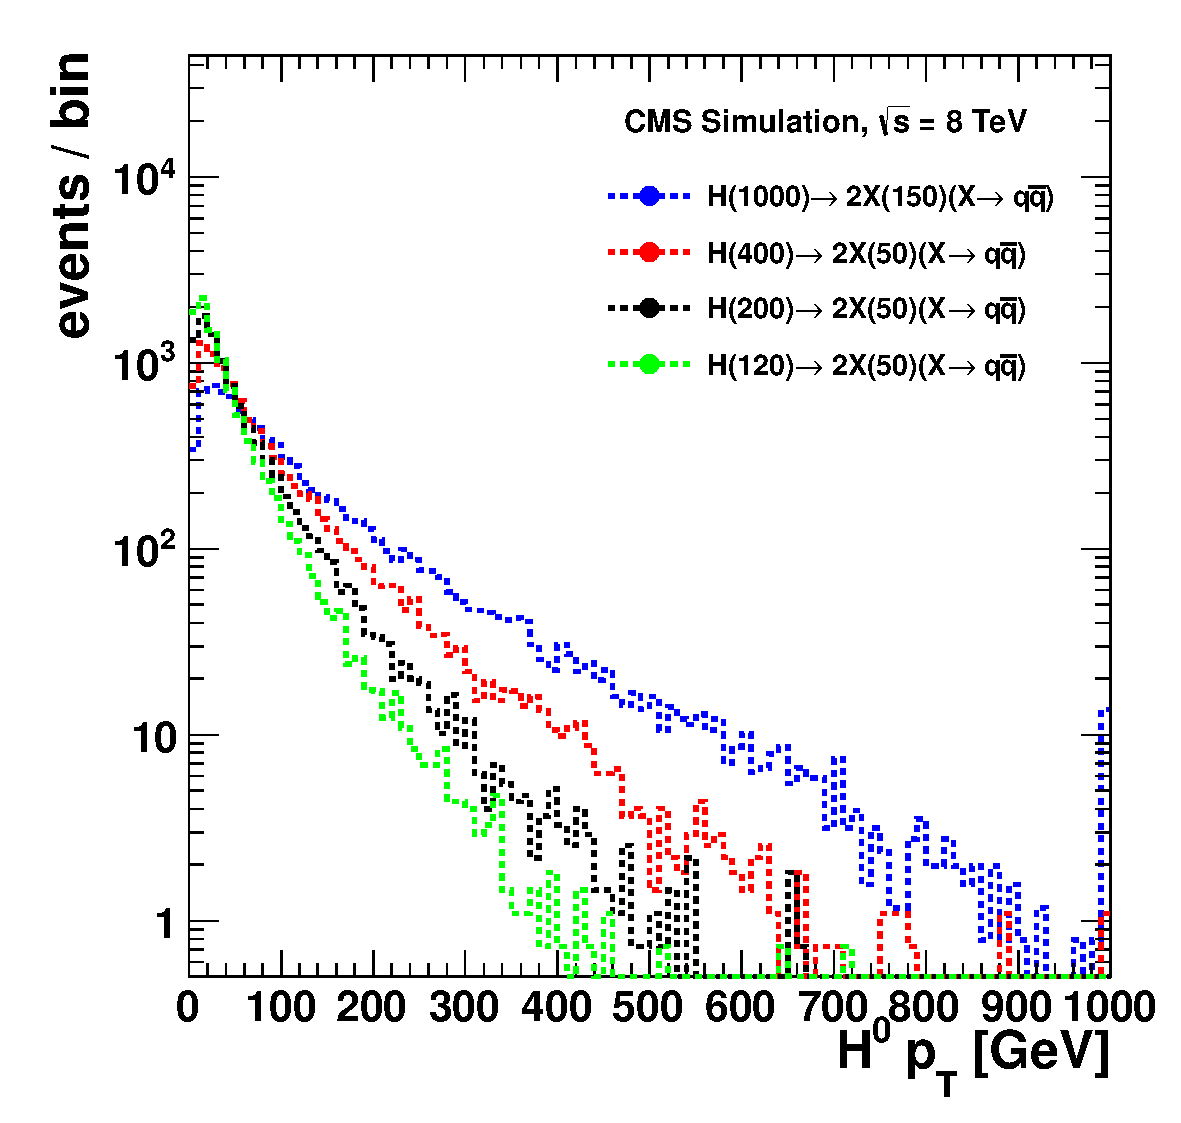
\includegraphics[width=0.495\textwidth]{plots/signal/hpt.pdf}
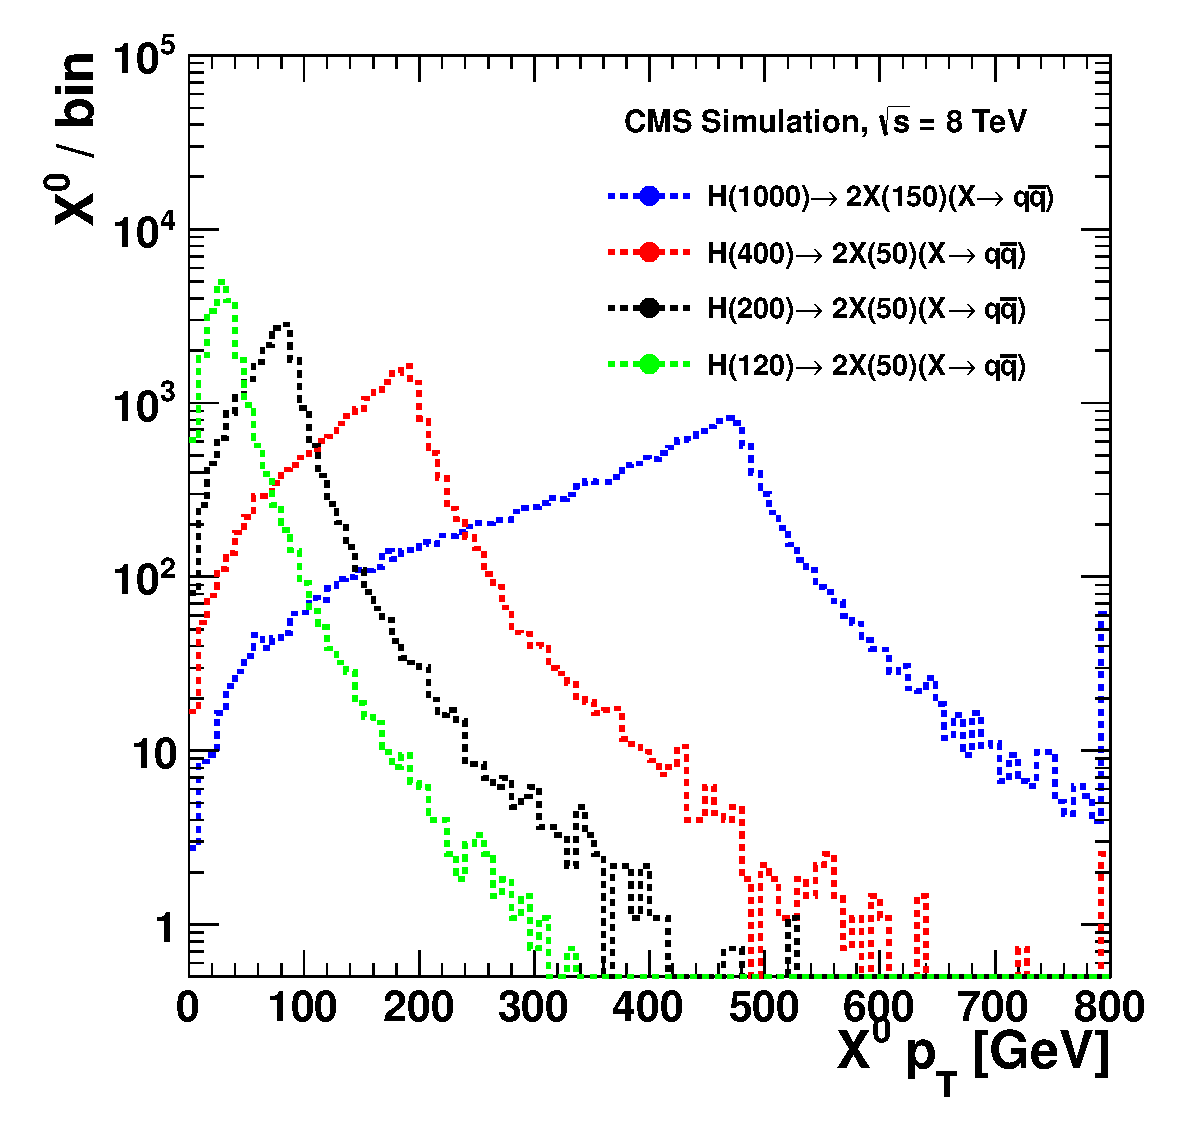
\includegraphics[width=0.495\textwidth]{plots/signal/xpt.pdf}
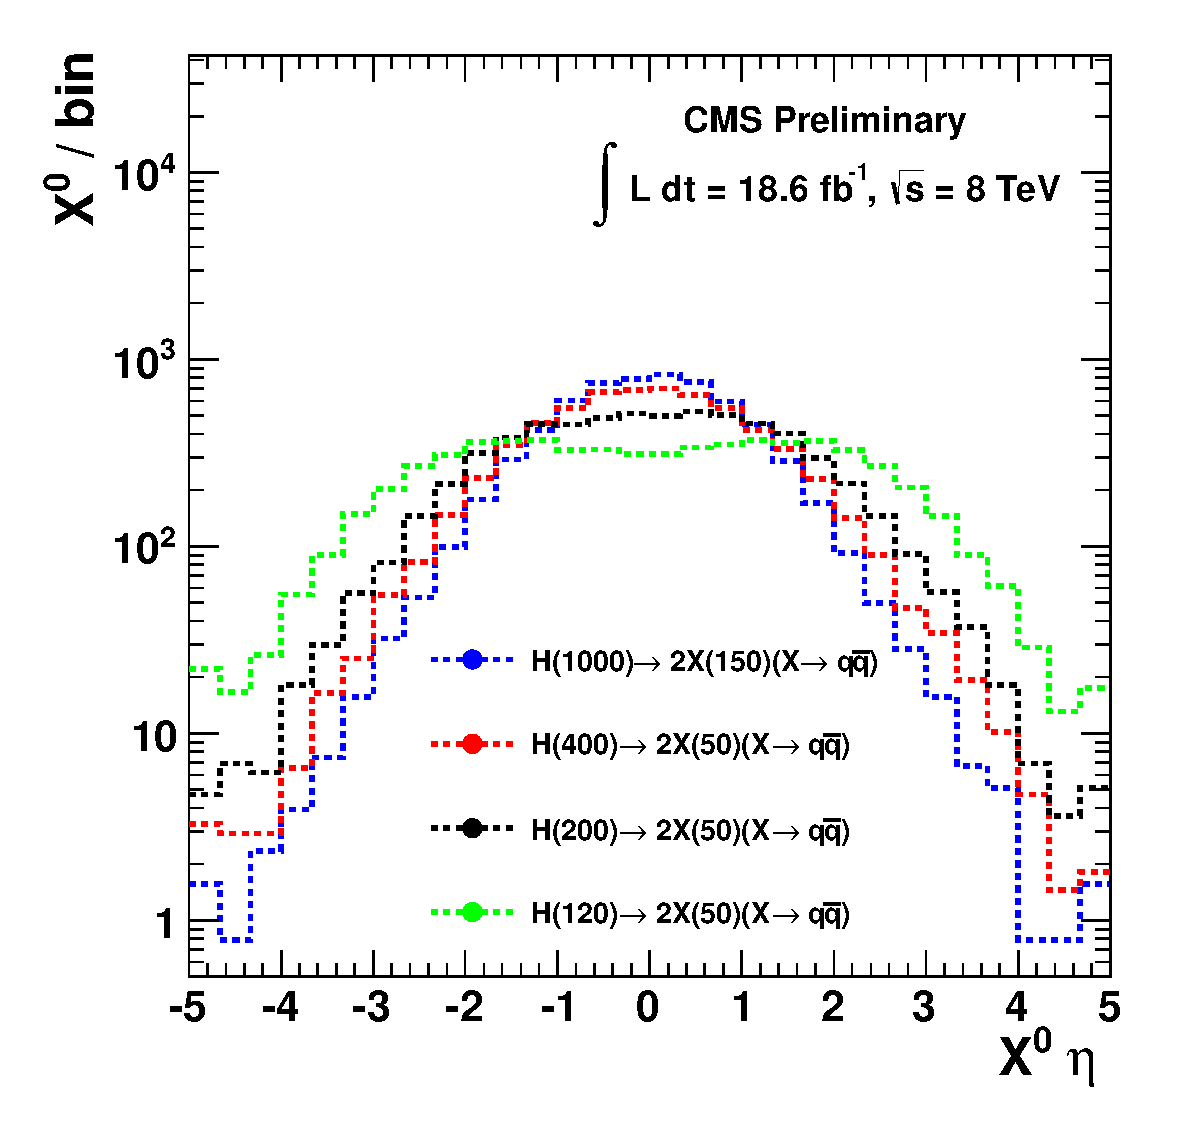
\includegraphics[width=0.495\textwidth]{plots/signal/xeta.pdf}
\caption{Generated \Higgs $p_T$ and \X $p_T$ and $\eta$ distributions for selected signal models.\label{fig:sigHX}}
\end{figure} 

The only significant background is expected to arise from QCD events, and the corresponding simulated samples
are listed in Table~\ref{tab:backgrMC}.
For each simulated background sample the number of events passing the signal trigger
scaled to the total integrated luminosity is shown. The per event weight factors that are applied according to the
number of events available in each sample are also given. The weight factors for samples with $\hat{p_T}$ 
below 470\GeV are significantly above 1, therefore the amount of simulated events in this region is insufficient. 
The background contribution   
significantly decreases with increased $\hat{p_T}$, therefore we do not consider samples with $\hat{p_T}$ higher
than 800 \GeV. For QCD events with $\hat{p_T}$ below 80\GeV the small efficiency of passing the trigger
 requirement of $H_T>$300\GeV 
makes the low $\hat{p_T}$ contribution negligible.  
In all the samples, the response of the detector is simulated
in detail using \GEANTfour~\cite{GEANT4}. The samples are then processed through the trigger emulation and
event reconstruction chain of the CMS experiment. An example event display of a reconstructed 
simulated signal event is presented in Figure \ref{fig:eventDisplay}.

\begin{figure}[htbp]
\centering
 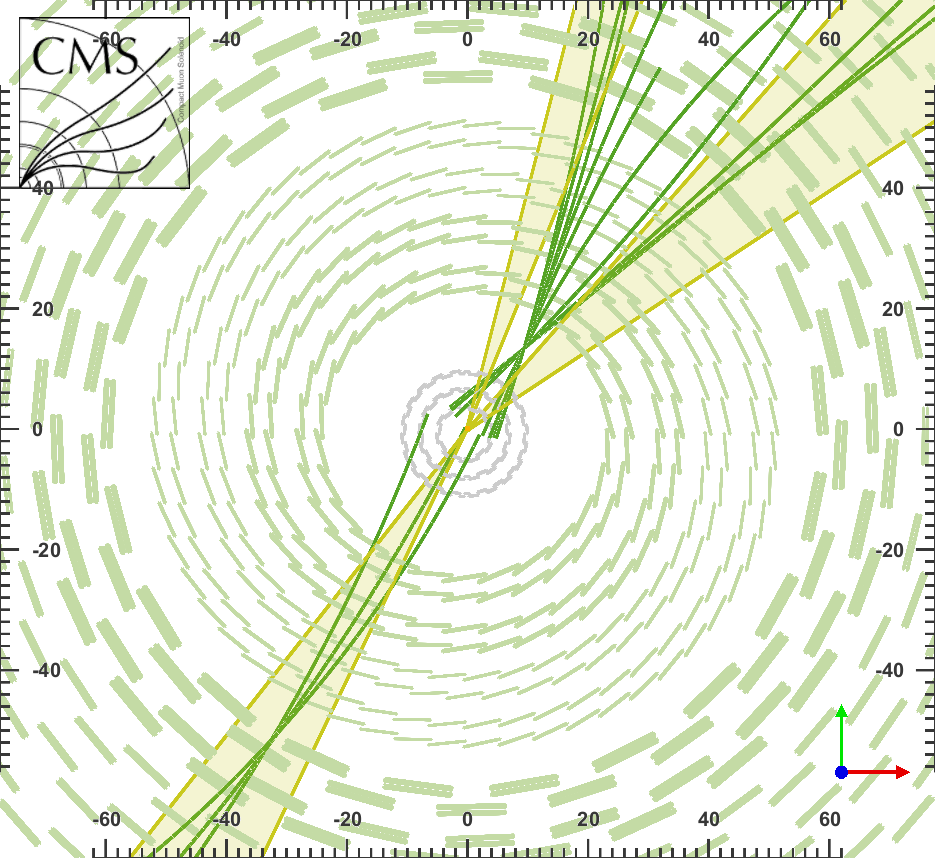
\includegraphics[width=0.6\textwidth]{plots/eventDisplay.png}
\caption{CMS event display of an example simulated signal event with a di-jet pair originating from a transversly displaced secondary vertex. \label{fig:eventDisplay}}
\end{figure}
 
\begin{table}[hbtp]
\begin{center}
\caption{Simulated signal samples used in the analysis. The masses of the \Higgs and \X bosons are given, 
as is the mean proper decay length of the \X~boson. \label{tab:signalMC}}
\begin{tabular}{|c|c|c|}
\hline 
  $M_{\Higgs}$ (\GeV) & $M_{\X}$ (\GeV) & $c\tau$ (cm) \\
\hline
       1000      &       350      &     3.5, 35, 350      \\          
       1000      &       150      &     1, 10, 100      \\          
       1000      &        50      &     0.4, 4, 40      \\          
       1000      &        20      &     0.15, 1.5, 15       \\          
       ~400      &       150      &     4, 40, 400      \\          
       ~400      &        50      &     0.8, 8, 80      \\          
       ~400      &        20      &     0.4, 4, 40      \\          
       ~200      &        50      &     2, 20, 200      \\          
       ~200      &        20      &     0.7, 7, 70      \\          
       ~120      &        50      &     5, 50, 500      \\          
       ~120      &        20      &     1.3, 13, 130      \\          
\hline
\end{tabular}
\end{center}
\end{table}


\begin{table}[hbtp]
\begin{center}
\caption{Simulated background samples used in the analysis.\label{tab:backgrMC}}.
\begin{tabular}{|l|c|c|c|}
\hline 
 \multicolumn{1}{|c|}{Dataset name} & Cross section  & Number of events passing  & Per event \\
                                    &     (pb)       & the trigger / 18.6 \fbinv & weight factor \\ 
\hline
\texttt{\small QCD\_Pt-600to800\_TuneZ2\_8TeV\_pythia6}               & 2.70e1       & 4.5e2 & 0.1  \\
\texttt{\small QCD\_Pt-470to600\_TuneZ2\_8TeV\_pythia6}               & 1.14e2       & 1.7e3 & 0.6 \\
\texttt{\small QCD\_Pt-300to470\_TuneZ2\_8TeV\_pythia6}               & 1.76e3        & 2.6e4 & 5.5 \\
\texttt{\small QCD\_Pt-170to300\_TuneZ2\_8TeV\_pythia6}               & 3.41e4 & 5.2e5 & 1.1e2 \\
\texttt{\small QCD\_Pt-120to170\_TuneZ2\_8TeV\_pythia6}               & 1.56e5  & 7.5e5 & 4.8e2 \\
\texttt{\small QCD\_Pt-80to120\_TuneZ2\_8TeV\_pythia6}                & 1.03e6  & 4.8e5 & 3.2e3 \\
\texttt{\small QCD\_Pt-50to80\_TuneZ2\_8TeV\_pythia6}                & 8.15e6  & 1.1e5 & 2.5e4 \\
\hline
\end{tabular}
\end{center}
\end{table}

